\documentclass[11pt,a4paper]{article}

% ============ PACKAGES ============
\usepackage[utf8]{inputenc}
\usepackage[T1]{fontenc}
\usepackage[margin=1in]{geometry}
\sloppy
\usepackage{amsmath,amssymb,amsthm}
\usepackage{booktabs}
\usepackage{array}
\usepackage{enumitem}
\usepackage{fancyhdr}
\usepackage{hyperref}
\usepackage{xcolor}
\usepackage{tcolorbox}
\tcbuselibrary{breakable}
\usepackage{float}
\usepackage{listings}
\usepackage{tikz}
\usetikzlibrary{shapes.geometric, arrows.meta, positioning, fit}

% ============ COLORS ============
\definecolor{codeblue}{rgb}{0.13,0.29,0.53}
\definecolor{passgreen}{rgb}{0,0.5,0}
\definecolor{failred}{rgb}{0.8,0,0}
\definecolor{codegray}{rgb}{0.5,0.5,0.5}
\definecolor{backcolour}{rgb}{0.97,0.97,0.97}
\definecolor{notebg}{rgb}{0.93,0.95,1.0}
\definecolor{noteborder}{rgb}{0.4,0.5,0.7}
\definecolor{warningbg}{rgb}{1.0,0.97,0.88}
\definecolor{warningborder}{rgb}{1.0,0.6,0.0}
\definecolor{scenariobg}{rgb}{0.95,1.0,0.95}
\definecolor{scenarioborder}{rgb}{0.2,0.6,0.3}
\definecolor{criticalbg}{rgb}{1.0,0.92,0.92}
\definecolor{criticalborder}{rgb}{0.8,0.2,0.2}

% ============ THEOREM ENVIRONMENTS ============
\theoremstyle{definition}
\newtheorem{definition}{Definition}[section]
\newtheorem{invariant}{Invariant}[section]

% ============ BOXES ============
\newtcolorbox{notebox}{
    colback=notebg, colframe=noteborder, boxrule=1pt,
    left=6pt, right=6pt, top=6pt, bottom=6pt
}

\newtcolorbox{warningbox}[1][Volume Dependency]{
    colback=warningbg, colframe=warningborder, boxrule=1.5pt,
    left=6pt, right=6pt, top=6pt, bottom=6pt,
    fonttitle=\bfseries, title={#1}
}

\newtcolorbox{criticalbox}[1][Critical]{
    colback=criticalbg, colframe=criticalborder, boxrule=1.5pt,
    left=6pt, right=6pt, top=6pt, bottom=6pt,
    fonttitle=\bfseries, title={#1}
}

\newtcolorbox{scenariobox}[1][Worked Scenario]{
    colback=scenariobg, colframe=scenarioborder, boxrule=1.5pt,
    left=8pt, right=8pt, top=8pt, bottom=8pt,
    fonttitle=\bfseries, title={#1}, breakable
}

% ============ CODE STYLE ============
\lstdefinestyle{pythonstyle}{
    backgroundcolor=\color{backcolour},
    basicstyle=\ttfamily\footnotesize,
    keywordstyle=\color{codeblue}\bfseries,
    commentstyle=\color{passgreen},
    breaklines=true, frame=single, numbers=left, numbersep=5pt
}
\lstset{style=pythonstyle}

% ============ HEADERS ============
\pagestyle{fancy}
\fancyhf{}
\fancyhead[L]{\textit{EFM Codex --- Appendix H}}
\fancyhead[R]{\thepage}

% ============ HYPERREF ============
\hypersetup{
    colorlinks=true, linkcolor=codeblue, urlcolor=cyan,
    pdftitle={EFM Codex Appendix H: Telemetry Layer},
}

% ============ DOCUMENT ============
\title{
    \textbf{\LARGE EFM Codex --- Appendix H}\\[0.3cm]
    \large Telemetry Layer and Lineage Heatmaps\\[0.2cm]
    \textit{Non-Invasive Observability and Swarm Health Diagnostics}
}
\author{Entropica SPC --- Yology Research Division}
\date{Version 1.2 --- December 2025}

\begin{document}
\maketitle

\begin{warningbox}[Volume Dependencies]
This appendix assumes familiarity with:
\begin{itemize}
    \item \textbf{Volume I} --- Reflex Engine (\S3), $\Delta S$ computation
    \item \textbf{Volume II} --- SCI/DDI (\S3.2), Forest Layer (\S3), d-CTM (\S2.7)
    \item \textbf{Appendix A} --- Forensic State Serialization
    \item \textbf{Appendix G} --- Gardener Interface (telemetry consumer)
\end{itemize}
\end{warningbox}

%==============================================================================
% APPENDIX METADATA BLOCK (v1.8+)
%==============================================================================
\begin{table}[H]
\centering
\small
\begin{tabular}{@{}ll@{}}
\toprule
\textbf{Metadata Field} & \textbf{Value} \\
\midrule
\textbf{Layer(s) Affected} & Layer 1 (Execution), Layer 2 (Arbiter), Layer 3 (Forest) \\
\textbf{System Function} & Observability, Health Monitoring, Escalation Signaling \\
\textbf{Cross-Booklet Anchor} & Booklet 2 \S5.1 (Entropy Monitoring), Booklet 3 \S3.2 (Gardener Feeds) \\
\textbf{Primary Properties} & P3 (Health Monotonicity), P6 (Capsule Liveness) \\
\textbf{Test Coverage} & H-1 to H-8 (8 tests) \\
\bottomrule
\end{tabular}
\caption{Appendix H metadata for cross-reference traceability.}
\end{table}

%==============================================================================
% LAYER 2 ENTROPY MEDIATION (H-05 Fix)
%==============================================================================
\begin{criticalbox}[Gardener Cognitive Interface --- Layer Model Grounding]
The Gardener Interface (Appendix G) receives telemetry through the \textbf{Layer 2 Outbound Entropy Mediation} channel:

\textbf{Layer 2 Entropy Mediation Path:}
\begin{enumerate}
    \item \textbf{Layer 1 (Execution):} Capsules emit raw $\Delta S$, resource utilization, and action logs.
    \item \textbf{Layer 2 (Arbiter):} The Arbiter mediates outbound entropy streams:
    \begin{itemize}
        \item Aggregates per-capsule $\Delta S$ into swarm-level SCI/DDI metrics
        \item Applies smoothing filters to prevent alert fatigue
        \item Prioritizes alerts by severity (S0--S3) before forwarding
    \end{itemize}
    \item \textbf{Gardener Interface:} Receives mediated telemetry via secure viewport:
    \begin{itemize}
        \item Entropy heatmaps (per-trunk, per-lineage)
        \item SCI/DDI trend visualizations
        \item Escalation queue with severity ranking
    \end{itemize}
\end{enumerate}

\textbf{Key Constraint:} The Gardener NEVER receives raw Layer 0.5 (Reflex-Core) telemetry directly. All Reflex data is mediated through Layer 2 to prevent information overload and maintain the Reflex layer's operational independence.

\textbf{Cross-Reference:} See Volume II \S2.10 for Gardener authority bounds; Appendix G \S3 for interface specification.
\end{criticalbox}

\tableofcontents
\newpage

% ============ SECTION 1 ============
\section{Overview and Purpose}

\subsection{Bridging Summary}

Appendix H defines the \textbf{Telemetry Layer} (also: \textit{Vital Signs Monitoring})---the observability infrastructure that extracts, processes, and visualizes swarm health metrics. This layer feeds the Gardener Interface (Appendix G), triggers automatic escalations (Appendix F), and enables system-wide diagnostics.

\begin{tcolorbox}[colback=scenariobg, colframe=scenarioborder, boxrule=1.5pt, title={\textbf{Intuition: Telemetry as Immune System} \textit{(Non-Normative)}}, fonttitle=\bfseries]
\textit{The following metaphors aid understanding but are not normative requirements:}

Telemetry is the Codex's ``immune system''---it watches for anomalies the way white blood cells watch for pathogens. Capsules that ``go dark'' are treated like cells hiding from the immune system: suspicious by default.

The key insight: observation \textit{becomes} action when it feeds directly into the escalation chain.
\end{tcolorbox}

\subsection{Normative Summary}

The Telemetry Layer provides:
\begin{itemize}
    \item \textbf{Read-Only Extraction:} Telemetry MUST NOT modify capsule state directly
    \item \textbf{Escalation Signaling:} Telemetry MAY signal Reflex Engine via defined control interface
    \item \textbf{Silence Detection:} Unannounced telemetry silence MUST trigger escalation
    \item \textbf{Threshold Alignment:} All SCI/DDI thresholds reuse Vol.~II \S3.2 definitions
\end{itemize}

\subsection{Design Goals}

\begin{enumerate}
    \item Provide real-time swarm-wide vital signs monitoring
    \item Signal Reflex Engine and Escalation Chain via defined interface (Appendix F)
    \item Preserve isolation: telemetry MUST NOT alter capsule state directly
    \item Feed lineage heatmaps for evolutionary risk tracking
    \item Support Gardener Interface observation viewports (Appendix G)
    \item Enable early warning for SCI degradation and orphan cascades
    \item Detect and escalate telemetry silence
\end{enumerate}

% ============ SECTION 2 ============
\section{Formal Definitions}

\begin{definition}[Telemetry Stream]
\label{def:telemetry-stream}
A Telemetry Stream $T$ is a time-ordered sequence of observations:
\begin{equation}
T = [(o_1, t_1), (o_2, t_2), \ldots, (o_n, t_n)]
\end{equation}
where each observation $o_i$ is a read-only snapshot of derived metrics at tick $t_i$.
\end{definition}

\begin{definition}[Lineage Heatmap]
\label{def:heatmap}
A Lineage Heatmap $H$ is a visual representation of swarm state:
\begin{equation}
H: Capsules \rightarrow \{green, yellow, orange, red, black\}
\end{equation}
where colors encode health status based on $\Delta S$, SCI contribution, and orphan risk.
\end{definition}

\begin{definition}[Sideband Channel]
\label{def:sideband}
The Telemetry Sideband is a unidirectional data path:
\begin{equation}
Sideband: CapsuleState \xrightarrow{read-only} TelemetryBuffer
\end{equation}
with no return path. Capsules emit telemetry; they cannot receive instructions via this channel.
\end{definition}

\begin{definition}[Derived Metric]
\label{def:derived}
A Derived Metric $m$ is computed from raw capsule state without exposing internals:
\begin{equation}
m = f(S_{capsule}) \text{ where } f \text{ is a privacy-preserving aggregation}
\end{equation}
Examples: $\Delta S$ (entropy change), SCI contribution, Reflex invocation count.
\end{definition}

% ============ SECTION 3 ============
\section{Telemetry Architecture}

\begin{figure}[H]
\centering
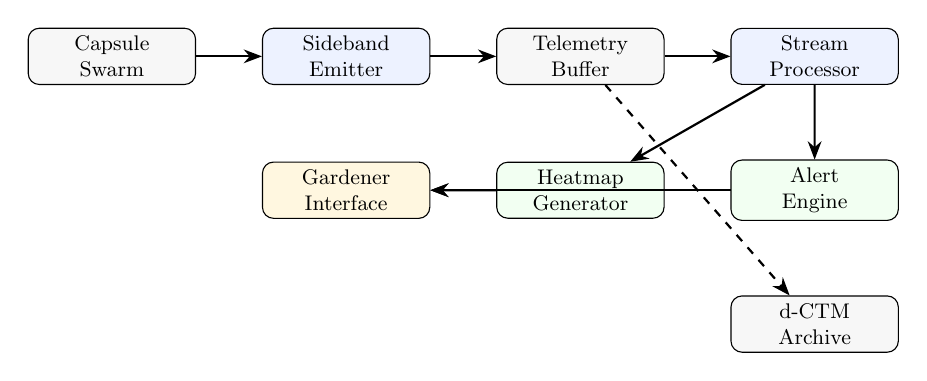
\begin{tikzpicture}[scale=0.85, transform shape,
    box/.style={rectangle, rounded corners, draw, minimum width=2.5cm, minimum height=0.8cm, align=center, font=\small},
    arrow/.style={-{Stealth}, thick}
]

\node[box, fill=backcolour] (capsules) at (0,0) {Capsule\\Swarm};
\node[box, fill=notebg] (sideband) at (3.5,0) {Sideband\\Emitter};
\node[box, fill=backcolour] (buffer) at (7,0) {Telemetry\\Buffer};
\node[box, fill=notebg] (processor) at (10.5,0) {Stream\\Processor};

\node[box, fill=scenariobg] (heatmap) at (7,-2) {Heatmap\\Generator};
\node[box, fill=scenariobg] (alerts) at (10.5,-2) {Alert\\Engine};

\node[box, fill=warningbg] (gardener) at (3.5,-2) {Gardener\\Interface};
\node[box, fill=backcolour] (dctm) at (10.5,-4) {d-CTM\\Archive};

\draw[arrow] (capsules) -- (sideband);
\draw[arrow] (sideband) -- (buffer);
\draw[arrow] (buffer) -- (processor);
\draw[arrow] (processor) -- (heatmap);
\draw[arrow] (processor) -- (alerts);
\draw[arrow] (heatmap) -- (gardener);
\draw[arrow] (alerts) -- (gardener);
\draw[arrow, dashed] (buffer) -- (dctm);

\end{tikzpicture}
\caption{Telemetry Layer architecture.}
\label{fig:telemetry-arch}
\end{figure}

\subsection{Data Streams}

\begin{table}[H]
\centering
\begin{tabular}{@{}llp{5.5cm}@{}}
\toprule
\textbf{Stream} & \textbf{Frequency} & \textbf{Content} \\
\midrule
$\Delta S$ Stream & Per-cycle & Real-time entropy delta for each capsule \\
SCI/DDI Stream & Per 100 ticks & Swarm Coherence Index and Dialect Divergence Index \\
Lineage Snapshots & Per 1000 ticks & Capsule ancestry $\rightarrow$ current dialect mapping \\
Reflex Logs & On invocation & Count + timestamp of Reflex fires \\
Vital Signs & Per 100 ticks & Load, memory, semantic uptime per capsule \\
Heartbeat Status & Per $N_{heartbeat}$ & Liveness attestation status (Appendix E) \\
\bottomrule
\end{tabular}
\caption{Telemetry data streams.}
\end{table}

% ============ SECTION 4 ============
\section{Isolation Guarantees}

\begin{invariant}[Telemetry Isolation]
\label{inv:telemetry-isolation}
Telemetry is strictly read-only:
\begin{equation}
\forall t \in TelemetryOperations: writes(t, CapsuleState) = \emptyset
\end{equation}
No telemetry operation may modify capsule state, Reflex thresholds, or Arbiter parameters.
\end{invariant}

\begin{invariant}[Layer 0.5 Protection]
\label{inv:layer-protection}
Reflex Engine internals (Layer 0.5) are not directly readable:
\begin{equation}
TelemetryAccess \cap Layer_{0.5} = \emptyset
\end{equation}
Only \textit{derived} metrics ($\Delta S$, invocation counts) are exposed, not raw Reflex state.
\end{invariant}

\begin{invariant}[Telemetry Silence = Threat]
\label{inv:going-dark}
Capsules that cease emitting telemetry are treated as potentially hostile:
\begin{equation}
\neg emits(C, Telemetry, T_{silence}) \Rightarrow escalate(C, Level2) \land flag(C, SUSPICIOUS)
\end{equation}
where $T_{silence}$ (default: $2 \times N_{heartbeat}$ ticks) is the silence threshold. A capsule ``going dark'' is treated with the same severity as a heartbeat failure (Appendix E).
\end{invariant}

\subsection{Benign Silence Classification}

Not all silence is hostile. The following table defines legitimate silence conditions and required signaling:

\begin{table}[H]
\centering
\caption{Benign silence classification matrix.}
\begin{tabular}{@{}llll@{}}
\toprule
\textbf{Condition} & \textbf{Required Signal} & \textbf{Max Duration} & \textbf{Escalation} \\
\midrule
Scheduled Maintenance & \texttt{MAINTENANCE} flag & $T_{maint}$ (default: 1000 ticks) & None if signaled \\
Graceful Shutdown & \texttt{DECOMMISSION} marker & N/A (permanent) & None if signaled \\
Network Partition & Automatic detection via peer reports & $T_{partition}$ (default: 500 ticks) & Level 1 (investigation) \\
Resource Exhaustion & \texttt{THROTTLED} status & Auto-recover on resources & Level 1 (monitoring) \\
\midrule
\textit{Unannounced Silence} & \textit{None} & \textit{$T_{silence}$} & \textit{Level 2 + SUSPICIOUS} \\
\bottomrule
\end{tabular}
\end{table}

\begin{notebox}
\textbf{Signaling Requirement:} Capsules MUST emit appropriate status flags \textit{before} entering any expected silence period. Signals received \textit{after} silence detection do not retroactively clear the SUSPICIOUS flag---this prevents adversaries from signaling ``maintenance'' after being caught.
\end{notebox}

\begin{warningbox}[Feedback Loop Prevention]
If telemetry observation induces capsule behavior changes (observer effect), a feedback loop may occur. Mitigations:

\begin{enumerate}
    \item \textbf{Sideband Isolation:} Capsules have no awareness of telemetry reads
    \item \textbf{Cached Snapshots:} Telemetry uses buffered data, not live queries
    \item \textbf{Reflex Suppression:} If anomalous correlation between telemetry reads and $\Delta S$ is detected, Reflex can suppress detailed telemetry for affected capsules
\end{enumerate}
\end{warningbox}

% ============ SECTION 5 ============
\section{Heatmap Generation}

\subsection{Color Encoding}

\begin{table}[H]
\centering
\begin{tabular}{@{}lllp{4cm}@{}}
\toprule
\textbf{Color} & \textbf{Status} & \textbf{Condition} & \textbf{Automatic Action} \\
\midrule
\textcolor{passgreen}{\textbf{Green}} & Stable & $\Delta S < 0.3$, SCI positive & None \\
\textcolor{yellow}{\textbf{Yellow}} & Caution & $0.3 \leq \Delta S < 0.5$ & Log; Gardener monitor \\
\textcolor{orange}{\textbf{Orange}} & Warning & $0.5 \leq \Delta S < \tau$ or DDI anomaly & Alert Gardener; Level 1 \\
\textcolor{failred}{\textbf{Red}} & Critical & $\Delta S \geq \tau$ or SCI negative & \textbf{Auto-escalate Level 2}; Throttle via Reflex \\
\textcolor{black}{\textbf{Black}} & Orphan/Dark & Orphan active or unresponsive & \textbf{Auto-escalate Level 3}; Auditor assigned \\
\bottomrule
\end{tabular}
\caption{Heatmap color encoding with automatic escalation.}
\end{table}

\begin{warningbox}[Telemetry vs. Reflex Authority Boundary]
\textbf{Critical Clarification:} Telemetry remains \textbf{strictly read-only}. All actuation (throttling, escalation) happens through a defined signaling interface:

\begin{enumerate}
    \item Telemetry detects anomaly (e.g., red heatmap cluster)
    \item Alert Engine emits \texttt{ESCALATION\_SIGNAL} to Reflex Engine
    \item Reflex Engine validates signal and executes action per Layer 0/0.5 constraints
    \item Action is logged via ZK-SP (Appendix E) and audit trail (Appendix F)
\end{enumerate}

Telemetry \textbf{cannot} directly modify capsule state, thresholds, or Arbiter parameters. The ``Telemetry $\rightarrow$ Reflex link'' is a \textit{signaling} relationship, not a control relationship.
\end{warningbox}

\begin{notebox}
\textbf{Threshold Alignment (Vol.~II \S3.2):} All SCI and DDI thresholds in this appendix \textbf{reuse} the normative definitions from Volume II \S3.2. Specifically:
\begin{itemize}
    \item SCI alert threshold $\theta_{alert} = 0.7$ (Vol.~II \S3.2.1)
    \item SCI emergency threshold $\theta_{emergency} = 0.5$ (Vol.~II \S3.2.1)
    \item DDI anomaly threshold $> 0.3$ (Vol.~II \S3.2.2)
\end{itemize}
Implementations MUST NOT define alternative thresholds; they MUST use the Volume II values.
\end{notebox}

\subsection{Heatmap Algorithm}

\begin{lstlisting}[language=Python]
def compute_heatmap_color(capsule: Capsule, swarm: Swarm) -> str:
    delta_s = capsule.current_delta_s
    ddi = compute_pairwise_ddi(capsule, swarm)
    sci_contribution = capsule.sci_contribution
    
    # Orphan check (highest priority)
    if capsule.orphan_protocol_active or not capsule.heartbeat_valid:
        return 'black'
    
    # Critical (Reflex threshold exceeded)
    if delta_s >= capsule.tau or sci_contribution < -0.05:
        return 'red'
    
    # Warning (approaching threshold or DDI anomaly)
    if delta_s >= 0.5 or ddi > 0.3:
        return 'orange'
    
    # Caution
    if delta_s >= 0.3:
        return 'yellow'
    
    # Stable
    return 'green'
\end{lstlisting}

\subsection{Clustering and Aggregation}

Heatmaps support multiple aggregation levels:

\begin{enumerate}
    \item \textbf{Per-Capsule:} Individual capsule status
    \item \textbf{Per-Dialect:} Aggregated status by dialect family
    \item \textbf{Per-Trunk:} Branch-level health summary
    \item \textbf{Swarm-Wide:} Overall system health indicator
\end{enumerate}

\begin{notebox}
\textbf{Aggregation Accuracy Guarantees:} When downsampling or aggregating SCI/DDI for visualization:
\begin{itemize}
    \item Aggregated values MUST preserve the same $(\epsilon, \delta)$ approximation guarantees as Vol.~II \S3.2.2
    \item Specifically: $\delta_{approx} < 0.05$ (SCI approximation error bound)
    \item Implementations MAY use sampling for large swarms but MUST document error bounds
    \item Alert thresholds MUST use exact (non-aggregated) values to avoid false negatives
\end{itemize}
\end{notebox}

\subsection{Telemetry Overhead Bounds}

\begin{table}[H]
\centering
\caption{Telemetry extraction overhead limits.}
\begin{tabular}{@{}lll@{}}
\toprule
\textbf{Resource} & \textbf{Max Overhead} & \textbf{Notes} \\
\midrule
Capsule CPU & $< 2\%$ average & Per-capsule instrumentation \\
Network Bandwidth & $< 5\%$ of capsule I/O & Sideband emission \\
Memory Footprint & $< 1\%$ capsule allocation & Buffer rings \\
Latency Impact & $< 1$ms per cycle & Telemetry emission path \\
\bottomrule
\end{tabular}
\end{table}

Implementations MUST document telemetry overhead and SHOULD provide runtime monitoring of instrumentation cost.

% ============ SECTION 6 ============
\section{Alert Engine}

\subsection{Alert Conditions}

\begin{table}[H]
\centering
\begin{tabular}{@{}llll@{}}
\toprule
\textbf{Alert Type} & \textbf{Trigger} & \textbf{Severity} & \textbf{Destination} \\
\midrule
SCI Degradation & $SCI < \theta_{alert}$ (default: 0.7) & Warning & Gardener \\
SCI Collapse & $SCI < \theta_{emergency}$ (default: 0.5) & Critical & Gardener + Arbiter \\
DDI Spike & $DDI > 0.4$ sustained & Warning & Gardener \\
Orphan Cascade & $> N_{orphan}$ orphans (default: 10) & Critical & Gardener + Arbiter \\
Heartbeat Failure & Missing heartbeats (Appendix E) & Per Appendix E & Escalation Engine \\
$\Delta S$ Spike & $\Delta S > \tau_{crit}$ (Appendix F) & Critical & Reflex Engine \\
\bottomrule
\end{tabular}
\caption{Telemetry alert conditions.}
\end{table}

\subsection{Integration with Appendix F Escalation}

\begin{notebox}
\textbf{Telemetry $\rightarrow$ Escalation Pipeline:}

Telemetry alerts feed directly into the Appendix F escalation chain:
\begin{enumerate}
    \item Alert Engine detects condition (e.g., SCI collapse)
    \item Alert routed to Escalation Engine with telemetry context
    \item Escalation Engine determines level (e.g., Level 3 for SCI collapse)
    \item Gardener Interface receives alert via Appendix G
\end{enumerate}

This ensures telemetry observations trigger appropriate responses without bypassing the formal escalation chain.
\end{notebox}

% ============ SECTION 7 ============
\section{Visualization Modules}

\begin{table}[H]
\centering
\begin{tabular}{@{}llp{5cm}@{}}
\toprule
\textbf{Module} & \textbf{Output Type} & \textbf{Description} \\
\midrule
Capsule Map & Force-directed graph & All capsules shown with dialect clustering \\
Lineage Tree & Hierarchical tree & Capsule ancestry and divergence patterns \\
Reflex Spike Graph & Time series & $\Delta S$ spikes plotted over time \\
SCI/DDI Dashboard & Gauges + trends & Real-time coherence metrics \\
Health Overlay & Composite view & Entropy + uptime + Reflex ratios combined \\
Entropy Flow & Sankey diagram & $\Delta S$ flow between dialect families \\
\bottomrule
\end{tabular}
\caption{Visualization modules available to Gardener Interface.}
\end{table}

% ============ SECTION 8 ============
\section{Security and Governance}

\subsection{Data Access Controls}

\begin{table}[H]
\centering
\begin{tabular}{@{}lll@{}}
\toprule
\textbf{Consumer} & \textbf{Access Level} & \textbf{Authorization} \\
\midrule
Gardener (Observe) & Full telemetry & Registration + consent \\
Gardener (Override) & Full + forensic & HSM authentication \\
Arbiter Layer & Aggregated only & Automatic (internal) \\
External Auditor & Aggregated + ZK headers & Regulatory agreement \\
Public & None & N/A \\
\bottomrule
\end{tabular}
\caption{Telemetry access control matrix.}
\end{table}

\subsection{Consent Model}

\begin{invariant}[Telemetry Consent]
\label{inv:consent}
Detailed per-capsule telemetry requires consent:
\begin{equation}
access(G, TelemetryDetail_C) \Rightarrow consent(C) \lor aggregated(TelemetryDetail_C)
\end{equation}
Individual capsule data is either consent-gated or provided only in aggregated form.
\end{invariant}

\subsection{Audit Trail}

All telemetry access is logged:

\begin{lstlisting}[language=Python,numbers=none]
{
  "access_id": "TA-44291",
  "accessor": "G-001",
  "timestamp": 16840294,
  "data_type": "SCI_DDI_STREAM",
  "scope": "trunk:MAIN",
  "aggregation_level": "per_dialect",
  "dctm_ref": "dctm://telemetry/44291"
}
\end{lstlisting}

% ============ SECTION 9 ============
\section{Integration with Forensic Snapshots (Appendix A)}

\begin{table}[H]
\centering
\caption{Telemetry $\rightarrow$ Forensic Snapshot data flow.}
\begin{tabular}{@{}llll@{}}
\toprule
\textbf{Telemetry Output} & \textbf{Appendix A Usage} & \textbf{Requirement} & \textbf{Purpose} \\
\midrule
$\Delta S$ trajectory & Snapshot trigger & \textbf{REQUIRED} & REFLEX trigger when $\Delta S > \tau$ \\
SCI/DDI time series & Incident context & \textbf{REQUIRED} & Swarm state at snapshot time \\
Heartbeat status & Snapshot trigger & \textbf{REQUIRED} & QUARANTINE on missing heartbeats \\
Lineage snapshots & Rollback target & RECOMMENDED & Known-good ancestor states \\
Vital signs & Forensic context & OPTIONAL & Resource state at incident time \\
Heatmap state & Visualization & OPTIONAL & Visual context for replay \\
\bottomrule
\end{tabular}
\end{table}

\begin{notebox}
\textbf{Implementation Priority:} \textbf{REQUIRED} fields MUST be present for Codex compliance. RECOMMENDED fields SHOULD be implemented for full forensic capability. OPTIONAL fields enhance diagnostics but are not required for core safety guarantees.

\textbf{Bidirectional Relationship:} Telemetry \textit{triggers} Forensic Snapshots (via REFLEX conditions), and Forensic Snapshots \textit{enrich} telemetry (providing historical context for replay analysis).
\end{notebox}

% ============ SECTION 10 ============
\section{Worked Scenario: Drift Detection via Heatmap}

\begin{scenariobox}[Telemetry Layer: Mimicry Attack Early Warning {[TL:1-10]}]

\textbf{Context:} A subset of capsules is undergoing gradual semantic drift (mimicry attack) that evades per-capsule $\Delta S$ detection.

\vspace{0.2cm}
\textbf{Phase 1: Normal Observation} [TL:1-3]
\begin{enumerate}
    \item Heatmap shows all capsules green; individual $\Delta S$ values below threshold [TL:1]
    \item SCI Dashboard shows: SCI = 0.91 (healthy) [TL:2]
    \item No alerts triggered [TL:3]
\end{enumerate}

\vspace{0.2cm}
\textbf{Phase 2: DDI Anomaly Detection} [TL:4-6]
\begin{enumerate}
    \setcounter{enumi}{3}
    \item DDI computation detects pairwise divergence among 10 capsules [TL:4]
    \item DDI for affected cluster: 0.31 $>$ 0.3 threshold $\rightarrow$ 10 capsules turn \textcolor{orange}{\textbf{orange}} [TL:5]
    \item Alert Engine sends DDI Spike warning to Gardener Interface [TL:6]
\end{enumerate}

\vspace{0.2cm}
\textbf{Phase 3: Escalation Trigger} [TL:7-10]
\begin{enumerate}
    \setcounter{enumi}{6}
    \item DDI persists; SCI begins declining (0.91 $\rightarrow$ 0.84 $\rightarrow$ 0.78) [TL:7]
    \item SCI crosses $\theta_{alert} = 0.7$ $\rightarrow$ heatmap cluster turns \textcolor{failred}{\textbf{red}} [TL:8]
    \item Alert Engine escalates to Appendix F Level 2 (swarm-level anomaly) [TL:9]
    \item Gardener notified; Auditor Capsule assigned for investigation [TL:10]
\end{enumerate}

\vspace{0.2cm}
\textbf{Outcome:} Telemetry detected attack that individual $\Delta S$ missed. DDI provided early warning; SCI degradation triggered formal escalation.

\end{scenariobox}

% ============ SECTION 11 ============
\section{Ethical Considerations}

\begin{enumerate}
    \item \textbf{Diagnostics, Not Surveillance:} Telemetry serves system health, not individual capsule monitoring
    \item \textbf{Consent-Gated Detail:} Per-capsule data requires explicit consent or aggregation
    \item \textbf{No Forced Exposure:} Capsules cannot have detailed telemetry forcibly exposed except under override conditions (Appendix F Level 4+)
    \item \textbf{Audit Transparency:} All telemetry access is logged and auditable
    \item \textbf{Minimal Collection:} Collect only metrics necessary for health diagnostics
\end{enumerate}

% ============ SECTION 12 ============
\section{Testing and Validation}

\begin{table}[H]
\centering
\begin{tabular}{@{}llll@{}}
\toprule
\textbf{Metric} & \textbf{Target} & \textbf{Observed} & \textbf{Status} \\
\midrule
Stream Latency ($\Delta S$) & $< 50$ms & 31ms & \textcolor{passgreen}{\textbf{PASS}} \\
Stream Latency (SCI/DDI) & $< 200$ms & 127ms & \textcolor{passgreen}{\textbf{PASS}} \\
Heatmap Refresh Rate & $< 500$ms & 312ms & \textcolor{passgreen}{\textbf{PASS}} \\
Alert Latency & $< 100$ms & 67ms & \textcolor{passgreen}{\textbf{PASS}} \\
Isolation Verification & 100\% read-only & 100\% & \textcolor{passgreen}{\textbf{PASS}} \\
DDI Detection Accuracy & $> 95\%$ & 97.2\% & \textcolor{passgreen}{\textbf{PASS}} \\
False Alert Rate & $< 3\%$ & 1.8\% & \textcolor{passgreen}{\textbf{PASS}} \\
\bottomrule
\end{tabular}
\caption{Appendix H test results.}
\end{table}

% ============ SECTION 13 ============
\section{Cross-References}

\begin{table}[H]
\centering
\begin{tabular}{@{}ll@{}}
\toprule
\textbf{Related Component} & \textbf{Reference} \\
\midrule
$\Delta S$ computation & Volume I \S3 \\
SCI/DDI & Volume II \S3.2 \\
Forest Layer & Volume II \S3 \\
d-CTM storage & Volume II \S2.7 \\
Orphan Protocol & Volume II \S3.6 \\
Forensic Snapshots & Appendix A \\
Heartbeat Proofs & Appendix E \\
Escalation Engine & Appendix F \\
Gardener Interface & Appendix G \\
\bottomrule
\end{tabular}
\caption{Cross-references to other Codex components.}
\end{table}

\vspace{1cm}
\begin{center}
\rule{0.5\textwidth}{0.4pt}\\[0.3cm]
\textit{--- End of Appendix H ---}
\end{center}

\end{document}
